\documentclass[12pt,a4paper]{article}
\usepackage{vmargin}
\setmarginsrb{1.0in}{1.0in}{1.0in}{1.0in}{0mm}{0mm}{0mm}{10mm}

\usepackage{amsfonts,amsmath,amssymb}
\usepackage{amsthm}
\usepackage{graphicx}
\usepackage{amsmath}
\usepackage{xcolor}
%\usepackage{ngerman}
\usepackage{listings}
\usepackage[utf8]{inputenc}
%\usepackage[T1]{fontenc}
\usepackage{comment}
\usepackage{algorithm}
\usepackage{hyperref}
%%\usepackage{algpseudocode}
\renewcommand*\thealgorithm{}
\usepackage{algorithmic}
\usepackage{amsmath}

\newcommand{\N}{\mathbb{N}}
\newcommand{\R}{\mathbb{R}}
\renewcommand{\O}{\mathcal{O}}
\usepackage{mathtools}

\newtheorem{theorem}{Theorem}
\newtheorem{lemma}{Lemma}
\newtheorem{corollary}[theorem]{Corollary}
\newtheorem{conjecture}{Conjecture}
\newtheorem{fact}[theorem]{Fact}
%\newtheorem{proposition}[theorem]{Proposition}
\newtheorem{observation}{Observation}
%\newtheorem{notation}[theorem]{Notation}
\newtheorem{remark}{Remark}
\newtheorem{claim}{Claim}
\newtheorem{definition}{Definition}
%\theoremstyle{definition}
%\newtheorem{problem}[theorem]{Problem}
\newtheorem{example}{Example}
%\renewcommand{\qedsymbol}{\rule{1mm}{1mm}}
\newcommand\independent{\protect\mathpalette{\protect\independenT}{\perp}}
\def\thesection{\alph{section}}

\setlength{\parindent}{0pt}


\begin{document}

\noindent
\begin{minipage}{0.66\textwidth}
Hasso Plattner Institute Potsdam\\
\\
Seminar on Nature Inspired Algorithms\\ Summer 2017\\
Potsdam, \today
\end{minipage}
~
\begin{minipage}{0.30\textwidth}

\includegraphics[width=\textwidth]{Hasso_Plattner_Institut_Logo}
\end{minipage}


\begin{center}
 {\LARGE \textbf{Homework 1}}
 \vspace*{0.5cm}
\end{center}
%%%%%%%%%%%%%%%%%%%%%%%%%%%%%%%%%%%%%%%%%%%


%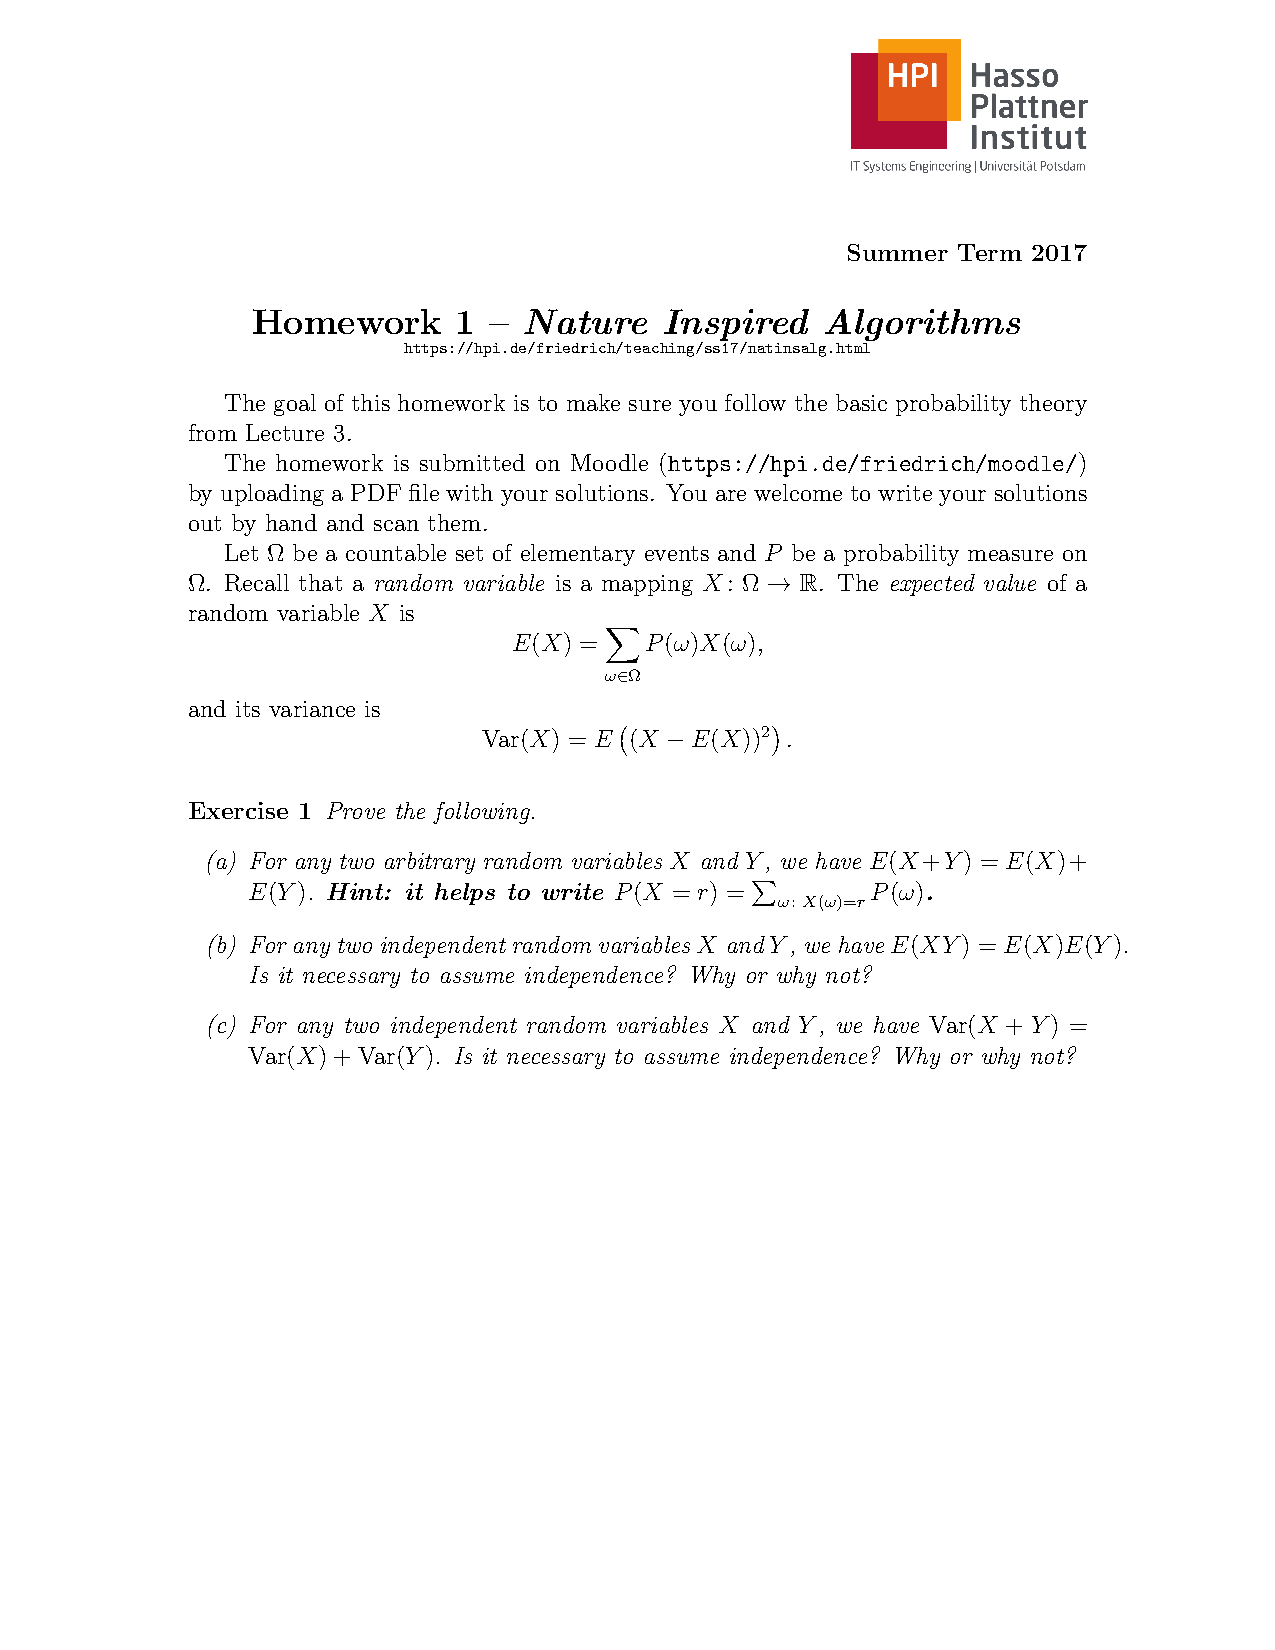
\includegraphics[clip, trim=0.5cm 2.5cm 0.5cm 4cm, width=0.99\textwidth]{homework01.pdf}

\section{}
\end{document}
